\mcchap{Analisi del sistema}{cap:cap2}
\section{Scopo del progetto}
L'obiettivo di questo progetto di tesi è quello di creare uno strumento 
per l'installazione rapida di patch di sicurezza in grado di sanare, 
nel più breve tempo possibile, vulnerabilità di livello critico sui 
sistemi operativi dei server.
Questo tool verrà quindi utilizzato dopo che una determinata 
vulnerabilità viene scoperta dal produttore del software (vendor), e dopo che 
il produttore avrà rilasciato una patch di sicurezza per risolvere la 
vulnerabilità.
\begin{figure}[H]
  \begin{flushright}
    \centering
    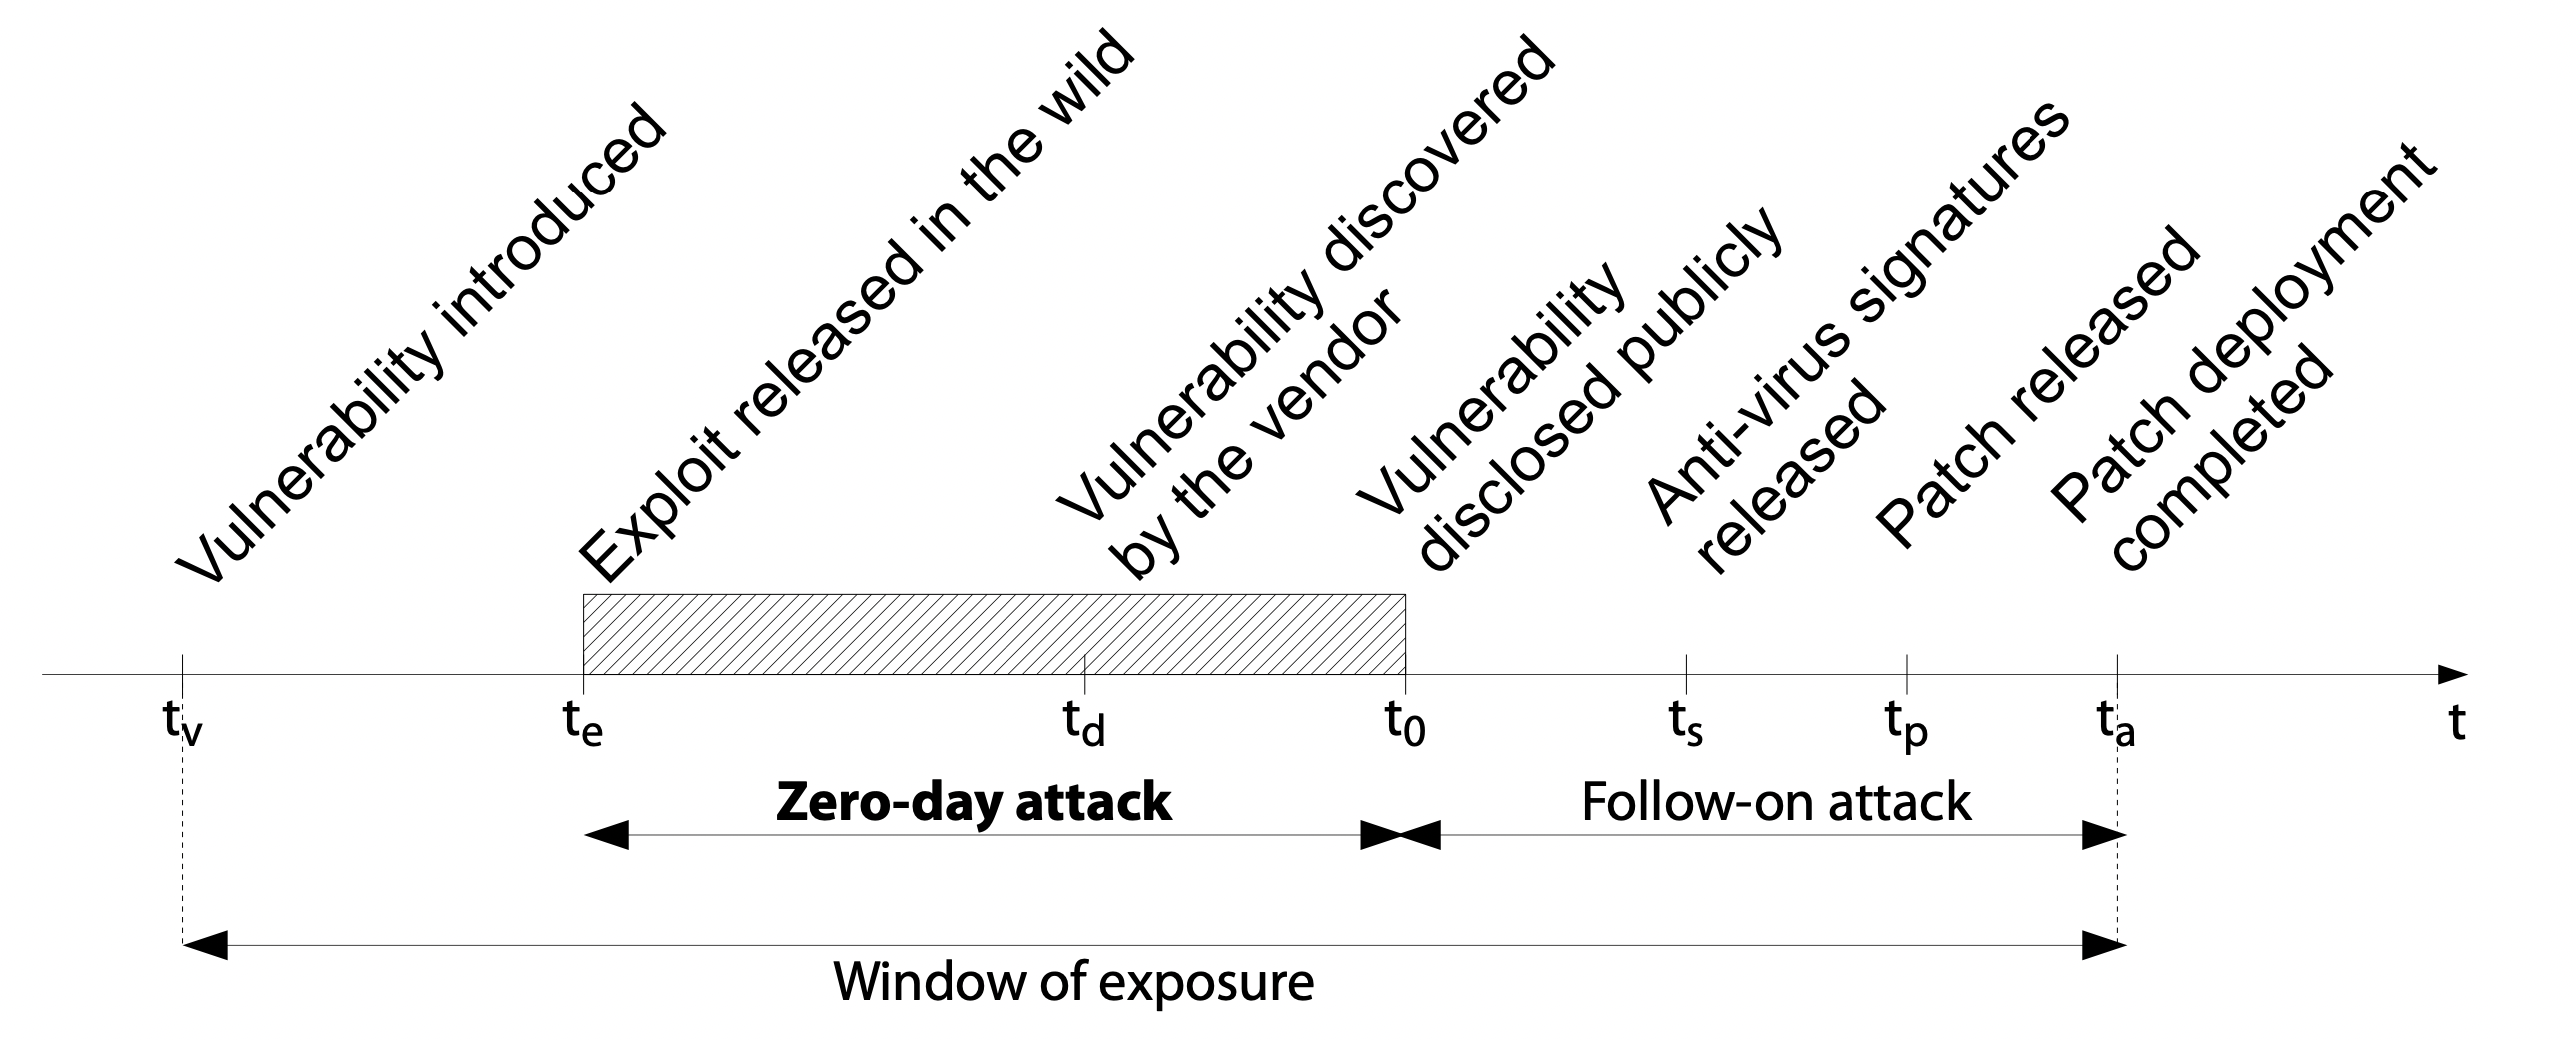
\includegraphics[width=0.90\textwidth]{imgs/vulnerability_windows.png}
    \caption{Sequenza degli eventi di una vulnerabilità}
    \label{fig:Sequenza degli eventi di una vulnerabilità}
  \end{flushright}
\end{figure}

In una tipica sequenza degli eventi di una vulnerabilità, le patch di 
sicurezza si installano a partire dal punto temporale tp 
(mostrato nella figura ~\ref{fig:Sequenza degli eventi di una vulnerabilità}), 
momento in cui il produttore rilascia al pubblico la risoluzione alla 
falla di sicurezza e inizia la campagna di aggiornamento, per risolvere la criticità. 
Durante questo periodo di patching (aggiornamento), che può durare anche 
mesi, il sistema, nella maggior parte dei casi, è ancora vulnerabile e 
solo una rapida installazione, della patch di sicurezza, può mettere il 
sistema informatico al riparo da un attacco che sfrutta quella falla.

Ed è proprio per installare rapidamente le patch di sicurezza che nasce 
l’Hotfix Response Center, nome ufficiale di questo progetto di tesi.
Lo scopo di questo strumento è quindi quello di gestire, in automatico, 
il patching straordinario di più server Linux o Windows Server che sono 
impattati dalla falla di sicurezza, per il quale è stata rilasciata 
la patch.
L’installazione delle patch di sicurezza avviene tramite la creazione 
di campagne di aggiornamento. Durante la creazione della 
campagna andranno specificati tutti i server impattati e dovranno essere 
caricate, all’interno del tool Hotfix, per ogni sistema operativo, le 
patch per risolvere le vulnerabilità, che il produttore avrà provveduto 
a rilasciare pubblicamente.

Questo strumento è indipendente da qualsiasi altro strumento ed è composto
da un’interfaccia grafica (frontend), da dei servizi REST (backend), da
un database dedicato, da uno storage per il caricamento delle patch e da
due script necessari all’installazione della patch di sicurezza, uno 
specifico per Windows, scritto in Powershell, e uno per Linux, scritto 
in bash.


\section{Funzionalità principali}
\subsection{Creazione di una campagna}
Una campagna di aggiornamento è un insieme di server, con diverso sistema 
operativo, che devono essere aggiornati, entro un periodo che va tra due e 
quattro settimane. 

\noindent Per creare una campagna occorre decidere:
\begin{itemize}
\item data e ora di inizio campagna;
\item data e ora di fine campagna;
\item elenco dei server impattati;
\item patch di sicurezza (rilasciate dal produttore del software) per 
ogni sistema operativo;
\end{itemize}
L’interfaccia grafica (frontend) per la creazione delle campagne sarà 
divisa in 3 step:
\begin{itemize}
\item Inserimento delle proprietà della campagna, tra cui: nome, data di 
inizio e fine, email del responsabile e tipologia della campagna 
(dettagliate più avanti).
\item Selezione dei server impattati: tramite le API (Application Program 
Interface) del gestionale in cui sono salvate tutte le informazioni dei 
server, si selezionano tutti i server impattati. L’interfaccia dovrà 
permettere di filtrare l’elenco completo dei server in base a: nome del
server, sistema operativo, indirizzo IP e tag associati ai server. 
Per tutti i server selezionati saranno poi recuperate tutte le informazioni
per consentire l’aggiornamento (dettagliate più avanti).
\item Caricamento delle patch: dopo aver selezionato tutti i server impattati,
per ogni sistema operativo selezionato, si dovrà caricare la patch di sicurezza 
da installare sui server.
\end{itemize}

\noindent Per ogni server da aggiornare bisogna recuperare, tramite le API del gestionale 
esterno, le seguenti proprietà:
\begin{itemize}
\item nome;
\item sistema operativo in uso;
\item indirizzo ip;
\item utenza di amministrazione per la connessione remota, utilizzata per 
installare le patch;
\item fascia di manutenzione: se presente indica le fasce orarie in cui il
server può essere aggiornato e riavviato. Ad esempio: MAR-MER-GIO(13:00-18:00)
indica che un server può essere aggiornato martedì, mercoledì e 
giovedì dalle 13 alle 18;
\item gruppo di patch: se presente impone che due o più server dello
stesso gruppo di patch non siano mai sotto manutenzione contemporaneamente. 
Questo per evitare problemi su applicazioni distribuite in cui tutti i server 
vengono aggiornati contemporaneamente. Chiamato con il campo restart group.
\item dipendenze: alcuni server devono essere aggiornati prima di altri. 
Ad esempio: i server di quality vanno aggiornati prima dei server di produzione.
Se un server ha una dipendenza bisogna fare in modo che durante l’aggiornamento
venga rispettata, garantendo almeno 24 ore tra una aggiornamento e l'altro.
\end{itemize}
Le credenziali per la connessione al server fornite devono essere funzionanti e con 
permessi di amministratore sulla macchina. Queste credenziali verranno usate
per la connessione remota al server.
Per consentire l’aggiornamento i server Windows devono avere WinRM abilitato.
Mentre i server Linux devono avere SSH attivo. WinRM è un protocollo di 
gestione usato da Windows per comunicare in remoto con un server. 
Si tratta di un protocollo che comunica su HTTPS, ed è incluso in tutti 
i recenti sistemi operativi Windows. Da Windows Server 2012, WinRM è 
abilitato di default. 
SSH, o Secure Shell, è un protocollo di amministrazione remota che consente 
agli utilizzatori di creare una connessione sicura con i server Linux.
WinRM e SSH verranno utilizzati attraverso Ansible per l’esecuzione di task
remoti. Il funzionamento di Ansible verrà approfondito nella sezione dedicata a 
pagina ~\pageref{subsec:Ansible}.

\noindent Le campagne possono avere due tipologie:
\begin{itemize}
\item standard: in cui vengono rispettate le fasce di manutenzione impostare 
per ogni server;
\item zero day: in cui tutti i server vengono schedulati per essere 
aggiornati il prima possibile.
\end{itemize}


\subsection{Schedulazione intelligente dei server}
Durante la creazione della campagna, quando si selezionano i server impattati 
dalla vulnerabilità di sicurezza, è possibile selezionare anche tutti i server
inseriti nel gestionale. 
È quindi necessario creare un algoritmo di schedulazione efficiente, capace di 
distribuire tutti i server da aggiornare, durante il periodo della campagna.
Tutte le campagne di aggiornamento durano tra due e quattro settimane. 
Ogni giorno viene diviso in più slot di 30 minuti. L’algoritmo di schedulazione 
dovrà essere in grado di trovare una schedulazione ottimale in base ai 
seguenti parametri:
\begin{itemize}
\item fascia di manutenzione corretta;
\item dipendenze tra server;
\item schedulare in modo da non avere due server con lo stesso 
“gruppo di patch” nello stesso slot;
\item schedulare in modo da avere massimo di server per slot, preferendo 
sempre slot vuoti. In una situazione ideale si schedula solo 1 server per slot.
\end{itemize}
L’algoritmo di schedulazione dovrà essere eseguito appena l’operatore, tramite 
l’interfaccia grafica, avrà inserito tutti i server da aggiornare nella 
campagna. L’algoritmo ha quindi pochi secondi per reperire le informazioni 
necessarie dei server e trovare la schedulazione migliore per la campagna.
Al termine dell’elaborazione verrà mostrato all’operatore un calendario con
tutte le schedulazioni di tutti i server nella campagna.
Attraverso il calendario della campagna dovrà essere possibile cambiare la 
data e/o l’ora di schedulazione, nel caso l’operatore ritenga opportuno
cambiare alcune schedulazioni.


\subsection{Caricamento file di aggiornamento}
Dopo l’inserimento di tutti i server vulnerabili, all'interno della campagna 
di aggiornamento, ci sarà un schermata di caricamento dei file di aggiornamento.
In questa schermata, per ogni differente sistema operativo dei server
selezionati, verrà dinamicamente mostrato l’elenco dei sistemi operativi
e un’interfaccia di caricamento per l’eseguibile/script di aggiornamento, 
da lanciare sulla macchina.
I file che saranno caricati dall’operatore saranno salvati in uno storage 
S3 dedicato.
Terminato il caricamento delle patch, per ogni sistema operativo, la campagna 
di aggiornamento può essere attivata dall’operatore.


\subsection{Avvio aggiornamento automatico}
La gestione degli aggiornamenti dei server dovrà essere automatica. 
Gli automatismi saranno gestiti con due cron jobs. I cron jobs sono 
dei programmi che vengono eseguiti ad orari prestabiliti. Cron è un programma di
utilità dei sistemi di tipo Unix che consente agli utenti di gestire 
le pianificazione di attività ripetute in un momento specifico.
La gestione automatica degli aggiornamenti sarà quindi gestita con 
dei task programmati che faranno partire l’aggiornamento sul server remoto.\\

\noindent Saranno presenti due cron job:
\begin{itemize}
\item job di avvio, schedulato ogni 30 minuti. Questo job seleziona tutte 
le campagne attive e farà partire gli aggiornamenti per i server schedulati 
in quello slot temporale. Ad esempio il job che parte alle 13:30 farà 
partire l’aggiornamento per i server schedulati dalle 13:30 alle 13:59; 
\item job di monitoraggio, schedulato ogni 10 minuti. Questo job monitorerà gli 
aggiornamenti in corso. Deve controllare che gli aggiornamenti automatici
procedano senza problemi rilevando se si verificano dei timeout 
(l’aggiornamento sta durando troppo oppure qualcosa si è interrotto 
senza preavviso). Questo job deve inoltre monitorare il corretto riavvio 
dei server dopo l’aggiornamento, per considerare l’aggiornamento 
come completato.
\end{itemize}


\subsection{Gestore dell’aggiornamento}
Un’ultima parte molto importante di questo sistema è lo script che gestirà 
l’aggiornamento sulla macchina remota. Ci saranno due diversi script: 
uno per i server Linux e uno per Windows server.
Lo script per Linux sarà realizzato in Bash mentre lo script per Windows 
server sarà realizzato in Powershell. Entrambi sono linguaggi di 
programmazione adatti per creare script iterativi da eseguire nella 
console dei rispettivi sistemi.
Il compito di questo script sarà quello di gestire l'aggiornamento del 
server remoto in modo automatico, comunicando con il server centrale lo 
stato dell’aggiornamento.
Lo scopo è quindi quello di scaricare la patch di aggiornamento dallo 
storage centrale e far partire l’aggiornamento sul server.
Per avere un maggiore controllo sullo stato di avanzamento lo script 
comunicherà gli stati intermedi durante l’operazione.\\

\noindent Gli stati che si susseguiranno durante l’operazione saranno:
\begin{itemize}
\item ping: test connessione all’avvio dello script; 
\item download patch: scaricamento dell’aggiornamento sul server;
\item esecuzione: installazione dell’aggiornamento;
\item reboot: riavvio del server, se necessario.
\end{itemize}
Al termine del riavvio il job di monitoraggio assegnerà lo stato 
completato. Se trascorre troppo tempo in uno step intermedio 
l’installazione andrà in timeout e l’aggiornamento sarà fallito.
La figura di pagina ~\pageref{fig:Diagramma a stati dell'aggiornamento di un server}
mostra il diagramma degli stati dell'aggiornamento.

\section{Diagramma delle attività}
La figura ~\ref{fig:Diagramma delle attività per la creazione di una campagna} 
rappresenta il diagramma delle attività per la creazione di una campagna di Hotfix.\\

\noindent Le entità coinvolte nella creazione sono:
\begin{itemize}
\item NIST (National Institute of Standards and Technology);
\item Il vendor del sistema operativo cioè colui che ha creato e gestisce il 
sistema operativo (Esempio Microsoft è il vendor di Windows);
\item Il tool Hotfix Response Center;
\item Il cliente.
\end{itemize}

Il flusso che porta alla creazione di una campagna di installazione 
parte dal NIST, l’ente americano che si occupa di gestire il National 
Vulnerability Database (NVD) fornendo punteggi CVSS per tutte le 
vulnerabilità note. Per quasi tutte le vulnerabilità, i vendor si preoccupano 
di fornire un patch, per sanare la vulnerabilità.
Il tool Hotfix Response Center è stato pensato per intervenire in situazioni 
d'emergenza, per patchare nel più breve tempo possibile le vulnerabilità critiche. 
Nel caso il CVSS (Common Vulnerability Scoring System) superi lo score di 9 su 
10 si controlla se tra i server dei clienti è presente la vulnerabilità appena scoperta.

Se i server dei clienti sono impattati si informa il cliente e, nel caso autorizzi 
l’aggiornamento straordinario, si procede con la creazione della campagna di 
aggiornamento per i server impattati dalla vulnerabilità.

Durante la creazione della campagna vengono caricate le patch di aggiornamento 
all’interno del tool e l’algoritmo di schedulazione cerca di trovare una 
schedulazione ottimale per patchare i server, nel più breve tempo possibile. 
Al termine di queste operazioni la campagna può essere avviata.

Sarà poi compito del cronjob di avvio, che parte ogni 30 minuti, controllare 
tutte le campagne attive e far partire l'aggiornamento automatico per i server 
schedulati nelle varie fasce d'orario.

\begin{figure}[H]
  \begin{flushright}
    \centering
    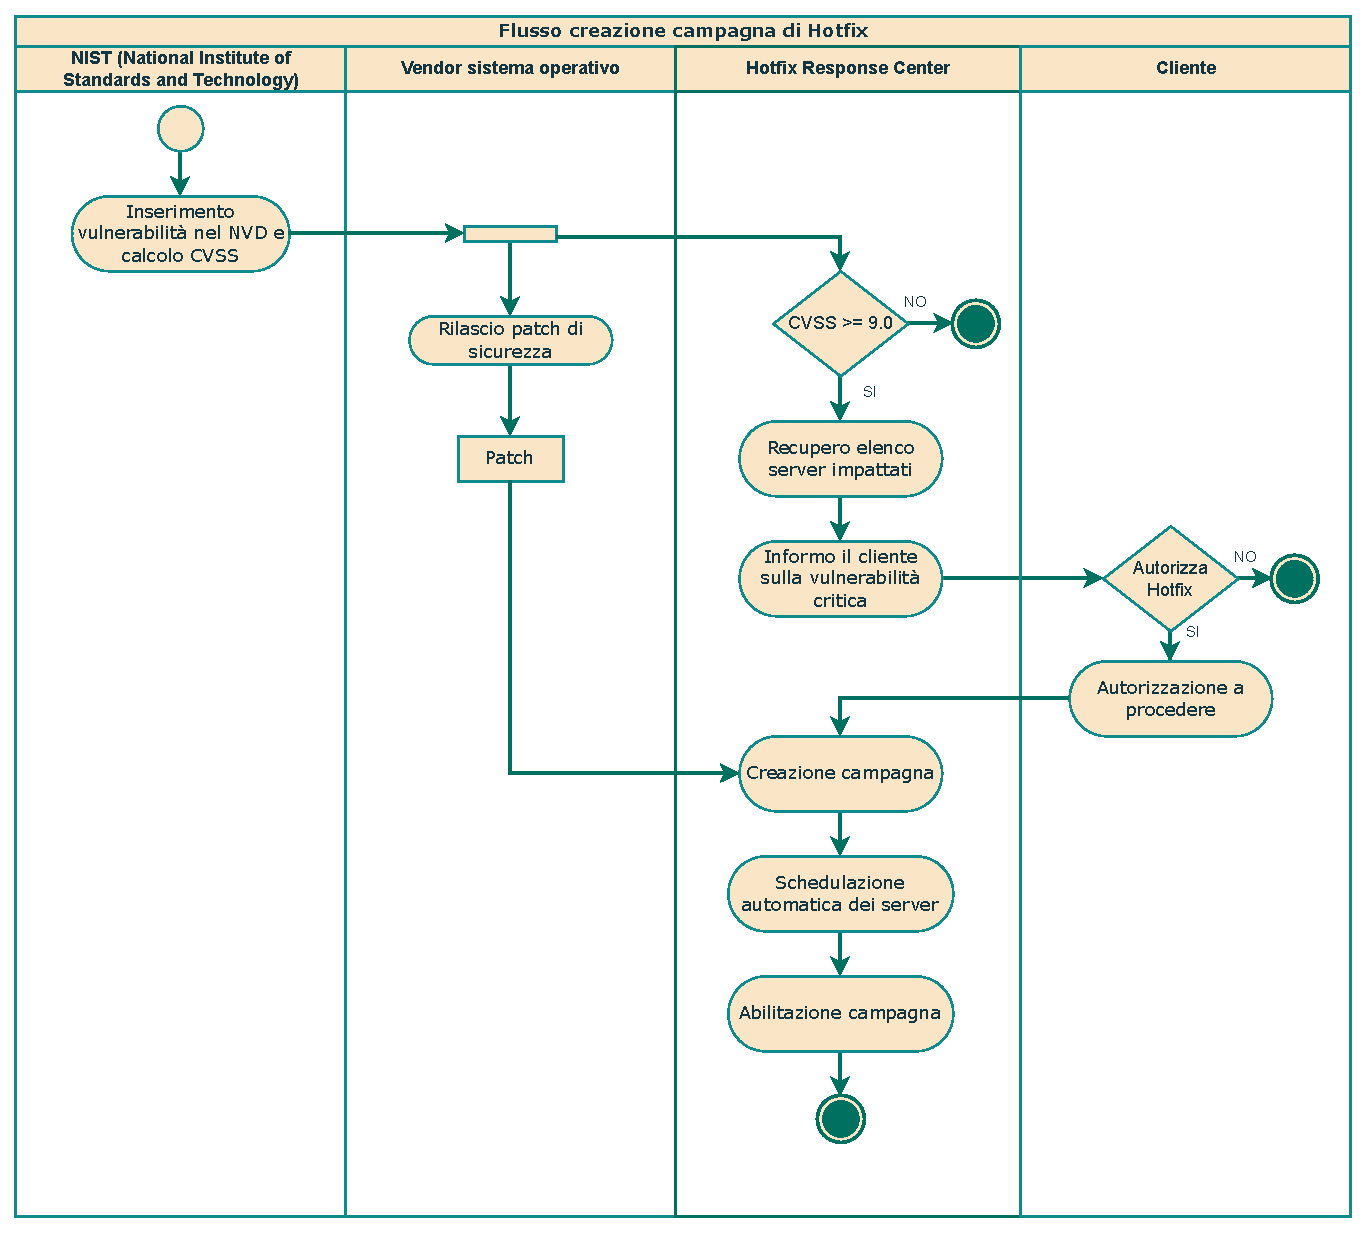
\includegraphics[width=0.98\textwidth]{imgs/hotfix_activity_diagram.pdf}
    \caption{Diagramma delle attività per la creazione di una campagna}
    \label{fig:Diagramma delle attività per la creazione di una campagna}
  \end{flushright}
\end{figure}
